%
%\input{tufte.inc}
%\input{symdef.inc}
\chapter{Kinematics} 
\label{ch:kinematics}
\section{Helmholtz's theorem}
\label{sec:helm}
Let us start with an experiment commonly performed by six year olds in
Sweden, we take a block of ``slime'' and deform it. Before deforming
we mark two point, $A$ and $B$,  on this slime with a different color. After the
deformation these two points have moved to two new positions. The
vector that connected these two points has also changed to a new
vector. Following Sommerfeld,~\cite{SomII06} I state the following: 
\marginnote{\input{bionotes/Sommerfeld}}
\begin{thm-non}
The most general motion of a sufficiently small element of a
deformable (i.e., not rigid) body can be represented as the sum of 
\begin{enumerate}
\item a translation
\item a rotation
\item an extension (contraction) in three mutually orthogonal
  directions. 
\end{enumerate}
\end{thm-non}
The original proof of this theorem is due to Helmholtz. 
The proof is based on Taylor series expansion as we describe below. 


Let us use a Cartesian coordinate system, in which the coordinates of 
a point $A$ are given by $x,y,z$. Under deformation every point in the
``slime'' moves to new position. Thus to every point in the dough I
can associate a vector $\uu$ which denotes the displacement of that
point under this deformation. This vector $\uu$ itself can then be
considered as a function of the three space coordinates
$x,y,z$. $\uu(x,y,z)$ is then a {\textit vector field}. 
You have encountered fields before, for example the temperature in
this room is a {\it scalar} field.  To imagine a scalar field think of
a number at every point in space. To imagine a vector field think of
an arrow associated with every point in space. A typical example of a
vector field will be a gravitational field. Consider a spec of
dirt. You take it to every point around the Earth and calculate the
gravitational force the earth exerts on it. Then divide the force by
the mass of the dirt to get force per-unit-mass. This is a vector that at
every point in space points towards the center of the Earth (if
Earth were a perfect sphere) and its magnitude decreases as the spec
of dirt is moved further and further away from Earth. Similarly we now
consider another vector field, that of displacement of material
points. Every point in the slime has been displaced: this displacement
itself, in general, is a function of position given by the vector field
$\uu$. Then consider two neighboring points $A(x,y,z)$ and
$B(x+\Delta x, y+\Delta y, z+\Delta z)$. Under deformation, $A$ 
moves to $\Ap$ and $B$ has moves to $\Bp$.
The vector $\overrightarrow{A\Ap}$ is given
by $\uu(x,y,z)$ and the vector $\overrightarrow{B\Bp}$ is given by $\uu(x+\Delta x,
y+\Delta y, z+\Delta z)$.  I can now expand each Cartesian component of the
vector field $\uu(x,y,z)$, given by $u_1(x,y,z)$, $u_2(x,y,z)$ and
$u_3(x,y,z)$, in a Taylor series\footnote{ This assumes that the field
  of displacement is ``smooth'' enough that the derivatives
  exists. This need not always be the case, for example,  if
  you deform the slime in a way that there is hole inside it then 
the displacement field may no longer be Taylor expandable. No such
case will be considered in these lectures. }
\begin{subequations}
\begin{align}
u_1(x+\Delta x, y+\Delta y, z+\Delta z) &= u_1(x,y,z) + \duxdx\Delta x
  + \duxdy \Delta y + \duxdz \Delta z + \ldots  \label{eq:ux}\\
u_2(x+\Delta x, y+\Delta y, z+\Delta z) &= u_2(x,y,z) + \duydx\Delta x
  + \duydy \Delta y + \duydz \Delta z + \ldots \label{eq:uy}\\
u_3(x+\Delta x, y+\Delta y, z+\Delta z) &= u_3(x,y,z) + \duzdx\Delta x
  + \duzdy \Delta y + \duzdz \Delta z + \ldots 
\end{align}
\label{eq:uu}
\end{subequations}
%
 \begin{marginfigure}
  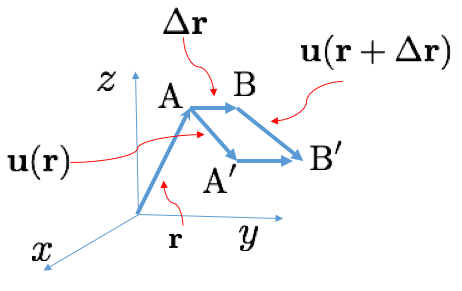
\includegraphics{figures/deform_sketch.png}
 \caption{We use a Cartesian coordinate system. In this system, the
   point A has the position vector $\rr$, and its neighboring point B
 has the position vector $\rr+\Delta \rr$. Under deformation A moves
 to ${\rm A}^{\prime}$ and B moves to ${\rm B}^{\prime}$. The
 deformation at A is $\uu(\rr)$ and the deformation at B is
 $\uu(\rr+\Delta \rr)$. }
  \label{fig:dsketch}
\end{marginfigure}
%
Let us compactify our notation. I use $\ua$ where $\alpha =1,2,3$ for
a component of the vector $\uu$. Let $\rr = (x,y,z)$ and $\Delta\rr =
(\Delta x, \Delta y, \Delta z)$. And I use the symbols 
\begin{subequations}
\begin{align}
a_{11} & =  \duxdx  \/, \quad a_{12} =  \duxdy \/,\quad  a_{13} =
         \duxdz \/, \\
a_{21} & =  \duydx  \/, \quad a_{22} =  \duydy \/,\quad  a_{23} =
         \duydz \/, \\
 a_{31} & =  \duzdx  \/, \quad a_{32} =  \duzdy \/,\quad  a_{33} =
         \duzdz \/,
\end{align} 
\end{subequations}
I can write the equation for deformation to be 
\begin{equation}
\ua(\rr) = \ua(\rr+\Delta \rr) + a_{\alpha\beta} \Delta r_{\beta} + \ldots
\end{equation}
\marginnote{
By $a_{\alpha\beta}\Delta r_{\beta}$ I mean
$\sum_{\beta=1,3}a_{\alpha\beta}\Delta r_{\beta}$. In these lectures
any index, e.g., $\beta$ here, that is repeated is assumed to be
summed -- this is known as the Einstein summation convention.  
}
Remember that the collection of number $a_{\alpha\beta}$ themselves
are function of space, they depend on \textit{where} we calculate the
derivatives.  As long as  $\mid\Delta \rr\mid$ is small enough I can
ignore all the higher order terms that I have denoted by the
triple-dots.  This is assumed in the rest of this discussion. 

\begin{fullwidth}
Now I am going to reorganize the collection of numbers
$a_{\alpha\beta}$ in ``symmetric'' and ``anti-symmetric'' manner: 
\begin{equation}
a_{\alpha\beta} = \frac{a_{\alpha\beta}-a_{\beta\alpha}}{2} +
  \frac{a_{\alpha\beta}+a_{\beta\alpha}}{2}  \/.
\label{eq:break}
\end{equation}
Substituting  back in \Eq{eq:uu} I get
\begin{subequations}
\begin{align}
u_1(\rr+\Delta \rr) &= u_1(\rr) + 
   {\color{red}0 + \frac{a_{12}-a_{21}}{2}\Delta y +
    \frac{a_{13}-a_{31}}{2}\Delta z}  +
       {\color{blue}a_{11}\Delta x+ \frac{a_{12}+a_{21}}{2}\Delta y +
    \frac{a_{13}+a_{31}}{2}\Delta z}\\
u_2(\rr+\Delta \rr) &= u_2(\rr) + 
   {\color{red}\frac{a_{21}-a_{12}}{2}\Delta x + 0 +
    \frac{a_{23}-a_{32}}{2}\Delta z}  +
       {\color{blue}\frac{a_{12}+a_{21}}{2}\Delta x+ a_{22}\Delta y +
    \frac{a_{23}+a_{32}}{2}\Delta z}\\
u_3(\rr+\Delta \rr) &= u_3(\rr) + 
   {\color{red}\frac{a_{31}-a_{13}}{2}\Delta x +
    \frac{a_{32}-a_{23}}{2}\Delta y+ 0}  +
       {\color{blue}\frac{a_{31}+a_{13}}{2}\Delta x+ 
    \frac{a_{23}+a_{32}}{2}\Delta y + a_{33}\Delta z}
\end{align}
\label{eq:u123}
\end{subequations}
\end{fullwidth}
I can now interpret the right-hand-side(RHS) of \Eq{eq:u123} 
as a sum of three displacements, 
\begin{equation}
\uu(\rr+\Delta \rr) = \dd_1+{\color{red}\dd_2}+{\color{blue}\dd_3}
\label{eq:disp}
\end{equation}
The black ones show that two neighboring points are
displaced by exactly the same amount, 
\begin{equation}
\uu(\rr+\Delta \rr) = \uu(\rr) \/,
\end{equation}
this is translation. 

Now organize the red ones
\begin{equation}
{\color{red}\dd_2  = 
\begin{pmatrix}
0 & \frac{a_{12}-a_{21}}{2} &
    \frac{a_{13}-a_{31}}{2}  \\
\frac{a_{21}-a_{12}}{2} &  0 &
    \frac{a_{23}-a_{32}}{2}  \\
\frac{a_{31}-a_{13}}{2} &
    \frac{a_{32}-a_{23}}{2} & 0 
\end{pmatrix}
\begin{pmatrix}
\Delta x \\ \Delta y  \\ \Delta z
\end{pmatrix}
 }
\label{eq:anti}
\end{equation}
The matrix the appears is an anti-symmetric matrix. 
%
 \begin{marginfigure}
  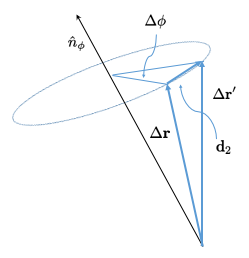
\includegraphics{figures/rotvec.png}
 \caption{Infinitismal rotation by cross-product. Write the vector $\Delta \pphi$
   as a vector pointing in the direction $\hat{n}_{\phi}$ with
   magnitude $\Delta \phi$.  The cross-product of $\Delta \pphi$ and
   $\Delta \rr$ is the vector $\dd_2$, and $\Delta \rr^{\prime} =
   \Delta \rr + \dd_2$. }
  \label{fig:rotvec}
\end{marginfigure}

A different but equivalent way to interpreting $\dd_2$ is 
\begin{equation}
\dd_2 = \frac{1}{2}\Delta \pphi \times \Delta \rr
\label{eq:rot}
\end{equation}
where the vector $\Delta \pphi \equiv (\Delta \phi_1,\Delta
\phi_2,\Delta \phi_3)$ is an infinitismal rotation vector
which points along the axis of rotation with a magnitude equal to the 
angle of rotation, with 
\begin{subequations}
\begin{align}
\Delta \phi_1 & =  a_{32}-a_{23} \/, \\
\Delta \phi_2 & =  a_{13}-a_{31} \/,\\
\Delta \phi_3 & =  a_{21}-a_{12} \/.
\end{align}
\end{subequations}
\marginnote{
An infinitismal rotation can be represented by a vector, although
not an ``usual'' vector but a \textit{axial} vector. Rotation by a
finite amount cannot in general be represented by a vector but 
can be represented by an anti-symmetric matrix 
as in \Eq{eq:anti}.
}
Let us now consider the blue terms in \Eq{eq:u123}
\begin{equation}
{\color{blue}\dd_3 = 
\begin{pmatrix}
a_{11} & \frac{a_{12}+a_{21}}{2} &
    \frac{a_{13}+a_{31}}{2}  \\
\frac{a_{21}+a_{12}}{2} &  a_{22} &
    \frac{a_{23}+a_{32}}{2}  \\
\frac{a_{31}+a_{13}}{2} &
    \frac{a_{32}+a_{23}}{2} & a_{33} 
\end{pmatrix}
\begin{pmatrix}
\Delta x \\ \Delta y  \\ \Delta z
\end{pmatrix}
}
\label{eq:sym}
\end{equation}

This is a real symmetric matrix. Hence it can always be diagonalized
by an orthogonal transformation. In other words, by a suitable
rotation of coordinates I can always find a new coordinate system in
which this matrix is diagonal. In that coordinate the displacement $\dd_3$
will have the form
\begin{equation}
{\color{blue}\dd_3 = 
\begin{pmatrix}
\Lambda_{1} & 0 & 0  \\
0 &  \Lambda_{2} & 0  \\
0 & 0 & \Lambda_{3} 
\end{pmatrix}
\begin{pmatrix}
\Delta X_1 \\ \Delta X_2  \\ \Delta X_3
\end{pmatrix}
}
\label{eq:diag}
\end{equation}
You may be already familiar with real symmetric matrices and their properties,
in particular their eigenvalues and eigenvectors from a course on
quantum mechanics where they appear as Hamiltonian or 
from a course in classical mechanics where they appear during the
discussions of moment of inertia of rigid objects. Proofs can be found
in any book on matrices or linear algebra, e.g., Arfken and Weber\cite{Arfken}.

The three $\Lambda$s are the three eigenvalues of the strain matrix
$s_{\alpha\beta}$ given in \Eq{eq:sym}. They must be real, but
they can be either positive or negative. A positive(negative)
$\Lambda$ denotes extension (compression) along the corresponding 
eigenvector $X$. The three eigenvectors are orthogonal to each other,
together they form a Cartesian triad. 
This proves Helmholtz's theorem. 

\section{Strain ellipsoid}
\label{sec:strain_ellipsoid}
One way to visualize the strain matrix is to construct what is called
its ``quadratic form'' , $f(x,y,z) \equiv
r_{\alpha}s_{\alpha\beta}r_{\beta} $
where the vector $\rr = (x,y,z)$ has components $r_{\alpha}$ with
$\alpha=1,2,3$. Written explicitly as
\begin{equation}
f(x,y,z) = 
\begin{pmatrix}
x & y & z 
\end{pmatrix}
\begin{pmatrix}
a_{11} & \frac{a_{12}+a_{21}}{2} &
    \frac{a_{13}+a_{31}}{2}  \\
\frac{a_{21}+a_{12}}{2} &  a_{22} &
    \frac{a_{23}+a_{32}}{2}  \\
\frac{a_{31}+a_{13}}{2} &
    \frac{a_{32}+a_{23}}{2} & a_{33} 
\end{pmatrix}
\begin{pmatrix}
x \\ y \\ z 
\end{pmatrix} 
\label{eq:ellipsoid}
\end{equation}
The function $f(x,y,z)$ is in general a quadratic in all its
arguments. Setting it equal to unity (or any other constant) defines a
surface in three dimensional space. This surface is called a {\textit strain
ellipsoid}. Geometrically, it is an actual ellipsoid only if all the
three eigenvalues of the strain matrix are positive.
% 
 \begin{marginfigure}
  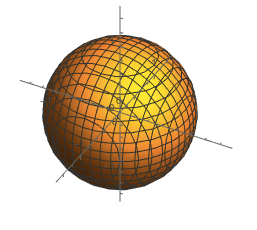
\includegraphics[width=0.8\textwidth]{figures/qsurf1.png}
  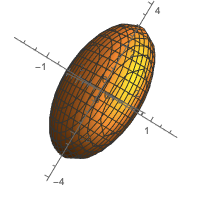
\includegraphics[width=0.8\textwidth]{figures/qsurf2.png}
  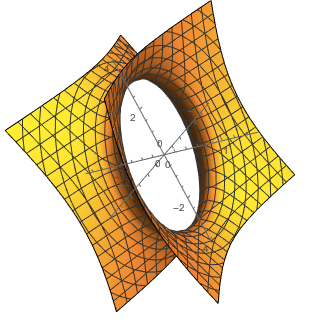
\includegraphics[width=0.8\textwidth]{figures/qsurf3.png}
 \caption{ Visualization of quadratic surfaces in three
   dimensions. The top one is a sphere with the equation
  $x^2+y^2+z^2=1$. The middle one is an ellipsoid 
  $4x^2+\frac{y^2}{4}+\frac{z^2}{9}=1$. The bottom one is
 $-4x^2+\frac{y^2}{4}+\frac{z^2}{9}=1$. These are the equations of
 these surfaces in terms of their eigencoordinates which are the axes
 shown in the figure. }
  \label{fig:qsurf}
\end{marginfigure}
%
A complete classification of quadratic surfaces can be found at 
\url{http://mathworld.wolfram.com/QuadraticSurface.html}. You should
use a visualization software  to play with quadratic
surface. The three simplest examples given in the margin are plotted
using Mathematica.
\section{Vorticity}
Let us now pass from displacement to velocity. We write the total
displacement $\uu$  as $\uu = \vv \Delta t$ and the infinitismal
rotation vector as $\Delta \pphi = \oo \Delta t$. In terms of
components this becomes 
\begin{subequations}
\begin{align}
u_1 = v_1 \Delta t \quad u_2 = v_2 \Delta t \quad u_3 = v_3 \Delta t
  \\
\Delta \phi_1 = \omega_1 \Delta t \quad \Delta \phi_2 =
  \omega_2 \Delta t\quad
  \Delta \phi_3 = \omega_3 \Delta t 
\end{align}
\end{subequations}
The vector $\oo$ is called the vorticity vector. You should
explicitly check that $\oo$ and  $\vv$ are related by  
\begin{equation}
\oo = \curl \vv
\end{equation}
The vorticity vector plays a crucial role in understanding the
behavior of fluids. 
\begin{Exercise}
\Question
To reinforce the idea that the displacement $\dd_2$ is indeed a
rotation show that under this displacement the length of the vector
$\Delta \rr$ remains unchanged. In particular, show that the two
vector $\Delta r$ and $\Delta r^{\prime}$ have the same length. 
\Question Consider the quadratic form in two variables
\begin{equation}
2x^2 + 5xy+ 3y^2 = 1
\end{equation}
Write this in a form similar to the RHS of \Eq{eq:ellipsoid}, you
should get a $2\times 2$ matrix. Diagonalize this matrix, find its
eigenvalues and eigenvectors. Sketch the two eigenvectors in the $x-y$
coordinate system. 
\end{Exercise}
\begin{subappendices}
\section{Who is afraid of Cartesian Tensors?}
I have so far interpreted the strain as a $3\times 3$ matrix at every
point in space. It is also viewed as a second rank tensor field. 
Any old collection of nine numbers at every point in space does not
make a tensor field, just like any collection of three numbers does
not make a vector field. They must satisfy the correct
\textit{transformation laws}. 
\marginnote{Here, by coordinate transformation I mean only rotation of
  coordinates. The transformation properties under
  more general, nonlinear coordinate transformation gives rise to more
  general non-Cartesian tensors -- they become useful while studying
  the general theory of relativity.}
 A scalar field, which a single number
at every point is space must be invariant under coordinate
transformation. A vector  does not remain invariant, but must change
exactly like (remain \textit{covariant})  the distance between two points
under coordinate transformation. A vector is a tensor of rank one, the
strain is a tensor of rank two. The vorticity can be either thought of
as a tensor of rank one, i.e., a vector but it is a \textit{polar}
vector, one that changes sign under the coordinate transformation
$x\to -x$, $y\to -y$ and $z\to -z$. Or it can be interpreted as a
second rank anti-symmetric tensor. In this course I assume you know
what a vector is, but not what a second or higher rank tensor is --
second or higher rank tensor are common occurrence in fluid mechanics,
I enthusiastically recommend a wonderful book by Rutherford
Aris~\cite{Aris} for a comprehensive introduction to this subject. 
During this course we shall learn tensors as and when we need them,
starting now. 

Consider a coordinate system $\{x_1,x_2,x_3\}$. We do a linear
transformation and obtain a new coordinate system
$\{y_1,y_2,y_3\}$. The linear transformation that relates them is give
by 
\begin{equation}
y_{\alpha} = a_{\alpha\beta} x_{\beta}\/,
\label{eq:transform}
\end{equation}
where $\alpha,\beta$ runs from $1$ to $3$ and we have again assumed
 the Einstein summation convention. A typical example is rotation about
 an axis, as shown in \Eq{eq:2drot}. 
\marginnote{
 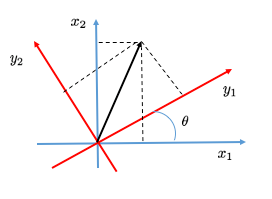
\includegraphics{figures/2drot.png} \\
An example of linear transformation of coordinates. The two
   Cartesian coordinate systems are related to each other by a
   rotation by the angle $\theta$ along an axis perpendicular to the
   plane. The same point in space are now labeled by two different
   coordinate systems $(x_1,x_2)$, and $(y_1,y_2)$ related to each
   other by 
\begin{equation}
\begin{pmatrix}
y_1 \\ y_2
\end{pmatrix}
=
\begin{pmatrix}
\cos\theta & -\sin\theta \\
\sin\theta & \cos\theta 
\end{pmatrix} 
\begin{pmatrix}
x_1 \\ x_2
\end{pmatrix}
\label{eq:2drot}
\end{equation}
 }
The magnitude of the position vector remains unchanged under rotation;
hence
\begin{equation}
y_{\alpha}y_{\alpha} = a_{\alpha\beta}a_{\alpha\mu} x_{\beta}x_{\mu}
= x_{\mu}x_{\mu} \/.
\end{equation}
Then we must have 
\begin{equation}
a_{\alpha\beta}a_{\alpha\mu} = \delta_{\beta\mu}
\label{eq:delta}
\end{equation}
where $\delta_{\beta\mu}$
\begin{equation}
\delta_{\beta\mu} =
\begin{cases} 1 \/, & \quad\quad {\rm for}\quad \beta = \mu \\
  0 \/,& \quad\quad {\rm otherwise}
\end{cases}
\end{equation}
is called the ``Kronecker delta''. You also know it as the identity matrix
\begin{equation}
\mathbb{1} = 
\begin{pmatrix}
1 & 0 \\
0 & 1
\end{pmatrix}
\end{equation}
Let us check \Eq{eq:delta} explicitly with the matrix $a_{\alpha\beta}$
given in \Eq{eq:2drot}:
\begin{subequations}
\begin{align}
\beta=1\/,\mu=1&\/ \quad\quad a_{11}a_{11} + a_{21}a_{21} =
  \cos^2\theta+\sin^2\theta = 1 \\
\beta=1\/,\mu=2&\/ \quad\quad a_{11}a_{12} + a_{21}a_{2} =
  \cos\theta\sin\theta-\cos\theta\sin\theta = 0 
\end{align}
\end{subequations}
\marginnote{ Multiply both sides of \Eq{eq:Ap} by $a_{\sigma\alpha}$ and sum over
the repeated index $\alpha$ to get
\begin{eqnarray}
a_{\alpha\sigma}\Ap_{\alpha} &=
  a_{\alpha\beta}a_{\alpha\sigma}A_{\beta}  \nonumber \\
\implies a_{\alpha\sigma}\Ap_{\alpha}&= \delta_{\beta\sigma}A_{\beta}
  = A_{\sigma} \nonumber \\
\implies A_{\alpha} &= a_{\beta\alpha}\Ap_{\beta} \/. \nonumber
\end{eqnarray}
In the second line above we have use \Eq{eq:delta}.
}
A vector is defined to be a quantity that transforms just like the
position vector under the same coordinate transformation, i.e., if any
vector $\AA= (A_1,A_2,A_3)$ in the coordinate system $(x_1,x_2,x_3)$
transforms to $\AAp = (\Ap_1,\Ap_2,\Ap_3)$ under the coordinate
transformation given in \Eq{eq:transform} then 
\begin{equation}
\Ap_{\alpha} = a_{\alpha\beta} A_{\beta}
\label{eq:Ap}
\end{equation}
We can invert \Eq{eq:Ap} to obtain
\begin{equation} 
 A_{\alpha} = a_{\beta\alpha}\Ap_{\beta} \/.
\label{eq:invert}
\end{equation}
In other words, the inverse of the matrix $a_{\alpha\beta}$ is its
transpose. This is a property of the rotation matrix that you may
already know. This is a consequence of demanding that the length of
vectors remain unchanged under the transformation \Eq{eq:transform}. 

Now let us try to find out how $s_{\alpha\beta}$ transforms
under the same coordinate transformation. Start with \Eq{eq:sym}
which we now write in compact notation as 
\begin{equation}
d_{\alpha} = s_{\alpha\beta}r_{\beta}
\end{equation}
Here for notational simplicity we have used $\rr$ instead of the
symbol $\Delta \rr$. 
As $\dd$ is a vector, its transform $\dd^{\prime}$ will satisfy an 
equation like \Eq{eq:invert}. Hence
\begin{equation}
a_{\mu\alpha}d^{\prime}_{\mu} = s_{\alpha\beta}r_{\beta}
\end{equation} 
Multiplying both sides by $a_{\kappa\alpha}$ and summing over the
repeated index $\alpha$ and subsequent simplification we obtain
\begin{equation}
d^{\prime}_{\kappa} =
  a_{\kappa\alpha}a_{\gamma\beta}s_{\alpha\beta}r^{\prime}_{\gamma}
\label{eq:ss}
\end{equation}
\marginnote{
The intermediate steps works out in the following manner:
\begin{eqnarray}
d_{\alpha} &= s_{\alpha\beta}r_{\beta} \nonumber \\
\implies a_{\mu\alpha}d^{\prime}_{\mu} &= s_{\alpha\beta}r_{\beta}
  \nonumber \\
\implies a_{\kappa\alpha}a_{\mu\alpha}d^{\prime}_{\mu} &=
  a_{\kappa\alpha}s_{\alpha\beta}r_{\beta} \nonumber \\
\implies \delta_{\kappa\mu}d^{\prime}_{\mu} &=
  a_{\kappa\alpha}s_{\alpha\beta}r_{\beta} \nonumber \\
\implies d^{\prime}_{\kappa} &=
  a_{\kappa\alpha}s_{\alpha\beta}r_{\beta} \nonumber \\
\implies d^{\prime}_{\kappa} &=
  a_{\kappa\alpha}a_{\gamma\beta}s_{\alpha\beta}r^{\prime}_{\gamma}
\nonumber
\end{eqnarray}
}
In the transformed (primed) coordinate system we should have 
\begin{equation}
d^{\prime}_{\kappa} = s^{\prime}_{\kappa\gamma}r^{\prime}_{\gamma}
\label{eq:sprime}
\end{equation}
Comparing \Eq{eq:ss} and \Eq{eq:sprime} we obtain the transformation
law for the strain
\begin{equation}
\boxed{s^{\prime}_{\kappa\gamma} = a_{\kappa\alpha}a_{\gamma\beta}s_{\alpha\beta}}
\end{equation}
We have now proved that the strain is a second rank tensor. In
general, any linear relationship between two vectors of the form
\begin{equation}
A_{\mu} = T_{\mu\nu}B_{\nu}
\label{eq:quotient}
\end{equation}
implies that the quantity $T_{\mu\nu}$ is a second rank tensor. 
This is sometimes called the ``quotient rule''. 
This is a very useful way to find out what kind of tensor a physical
quantity is. Two other examples where this rule is used are the moment of inertia tensor, or the polarizability
tensor of a medium. 

\subsection{Fully anti-symmetric tensor}
Let us revisit the displacement $\dd_2$
\begin{equation}
\dd_2  = 
\begin{pmatrix}
0 & \frac{a_{12}-a_{21}}{2} &
    \frac{a_{13}-a_{31}}{2}  \\
\frac{a_{21}-a_{12}}{2} &  0 &
    \frac{a_{23}-a_{32}}{2}  \\
\frac{a_{31}-a_{13}}{2} &
    \frac{a_{32}-a_{23}}{2} & 0 
\end{pmatrix}
\begin{pmatrix}
\Delta x \\ \Delta y  \\ \Delta z
\end{pmatrix}
\label{eq:anti2}
\end{equation}
where $a_{\alpha\beta} = \partial_{\beta} u_{\alpha}$.
In \Eq{eq:rot} we interpreted this equation as 
\begin{equation}
\dd_2 = (1/2) \Delta \pphi \times \Delta \rr 
\end{equation}
 To make a clearer connection to
vorticity let us write
\begin{equation}
\dd_2 = (1/2) \oo \times \Delta \rr \Delta t 
\end{equation} 
where 
\begin{equation}
\omega_1 = \partial_2v_3 - \partial_3v_2 \quad 
\omega_2= \partial_3v_1 - \partial_1 v_3 \quad 
\omega_3 = \partial_1v_2 - \partial_2 v_1 
\end{equation}
\marginnote{
I shall use either $\{x,y,z\}$ or $\{x_1,x_2,x_3\}$ or $\{x_{\mu}\}$ to denote
Cartesian coordinate systems.
I shall use bold fonts for vector, e.g., $\AA$, $\Delta \bm{r}$
etc. I shall write the individual components of the vector $\AA$ as
either $A_x,A_y,A_z$, or $A_1,A_2,A_3$ or collectively $A_{\mu}$. I
shall typically use Greek indices to denote components of vectors or
tensors. The convention can be extended in a straightforward way to
denote any component of a higher rank tensor, e.g., $T_{\alpha\beta}$
. Sometime I shall use the same symbol to denote the higher rank
tensor itself. The symbols $\frac{\partial}{\partial x}$,
$\partial_x$, $\partial_1$ will all mean the same thing, with the
symbol $\partial_{\mu}$ denoting partial derivative with respect to a
general coordinate $x_{\mu}$. 
}
Clearly,  \Eq{eq:anti2} can also be written as 
\begin{equation}
(d_2)_{\alpha} = (1/2)\Omega_{\alpha\beta} \Delta r_{\beta} \Delta t
\end{equation}
where  
\begin{equation}
\Omega_{\alpha\beta} = 
\begin{pmatrix}
0 & -\omega_3  & \omega_2 \\
\omega_3 & 0 & -\omega_1 \\
-\omega_2  & \omega_1 & 0 
\end{pmatrix}
\end{equation}
By the quotient rule the set of number $\Omega_{\alpha\beta}$ 
constitutes a second rank tensor, that is anti-symmetric. 
The vector $\oo$ and the second rank tensor $\Omega_{\alpha\beta}$ 
can be related to each other by, you guessed it, a \textit{third} rank
tensor :
\begin{equation}
\Omega_{\alpha\beta} = \epsilon_{\alpha\beta\gamma}\omega_{\gamma}
\end{equation}
This is called  the Levi-Civita tensor
\begin{equation}
\epsilon_{\alpha\beta\gamma} =
\begin{cases}
 0 \/,&\quad \text{ if any two of them are equal.} \\
1 \/,&\quad \text{ for even permutation} \\
-1 \/,& \quad \text{ for odd permutation}   
\end{cases} 
\end{equation}
\marginnote{
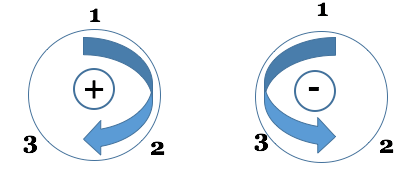
\includegraphics{figures/cross.png} \\
The only non-zero elements of $\epsilon_{\alpha\beta\gamma}$ are
\begin{eqnarray}
\epsilon_{123} &= \epsilon_{231}=\epsilon_{312} =1 
\nonumber \\
\epsilon_{132} &= \epsilon_{321}=\epsilon_{213} =-1 
\nonumber 
\end{eqnarray}
}
Using the  Levi-Civita tensor the cross-product of two vectors can be
written as
\begin{equation}
(\AA\times\BB)_{\alpha} = \epsilon_{\alpha\beta\gamma}A_{\beta}B_{\gamma}
\end{equation}
\end{subappendices}
%-------------
